% =============================================================================
% Personal notes on EEG streaming protocols
% InEar Teensy project
% =============================================================================
\documentclass[11pt,a4paper]{article}

% --- Packages ---
\usepackage[utf8]{inputenc}
\usepackage[T1]{fontenc}
\usepackage{lmodern}
\usepackage[margin=2.5cm]{geometry}
\usepackage{graphicx}
\usepackage{xcolor}
\usepackage{booktabs}
\usepackage{tabularx}
\usepackage{longtable}
\usepackage{array}
\usepackage{multirow}
\usepackage{makecell}
\usepackage{amsmath}
\usepackage{amssymb}
\usepackage{enumitem}
\usepackage{listings}
\usepackage{fancyvrb}
\usepackage{float}
\usepackage{caption}
\usepackage{subcaption}
\usepackage{textcomp}
\usepackage{hyperref}
\usepackage{cleveref}
\usepackage{tikz}
\usepackage{bytefield}
\usepackage{fancyhdr}
\usepackage{titlesec}
\usepackage{pifont}

% --- Colors ---
\definecolor{backgray}{HTML}{F7F7F7}
\definecolor{lightgray}{HTML}{D0D0D0}

% --- Listings setup ---
\lstdefinestyle{code}{
    backgroundcolor=\color{backgray},
    basicstyle=\ttfamily\small,
    breaklines=true,
    frame=single,
    rulecolor=\color{black},
    numbers=none,
    tabsize=4,
    showstringspaces=false,
    commentstyle=\itshape,
    keywordstyle=\bfseries,
    stringstyle={},
}

\lstdefinestyle{cpp}{
    style=code,
    language=C++,
    morekeywords={uint8_t, uint16_t, uint32_t, int32_t, int64_t, size_t, uint8__t},
}

\lstdefinestyle{diagram}{
    backgroundcolor=\color{backgray},
    basicstyle=\ttfamily\footnotesize,
    breaklines=false,
    frame=single,
    rulecolor=\color{black},
    numbers=none,
    tabsize=2,
    showstringspaces=false,
    literate={█}{{\textblock}}1
             {░}{{\textblock}}1
             {▼}{{$\blacktriangledown$}}1
             {▲}{{$\blacktriangle$}}1
             {✅}{{\ding{51}}}1
             {❌}{{\ding{55}}}1
             {⚠}{{$\triangle$!}}1,
}

\lstset{style=code}

% --- Custom commands ---
\newcommand{\tactic}[1]{\textbf{#1}}
\newcommand{\proto}[1]{\textsc{#1}}
\newcommand{\hexval}[1]{\texttt{0x#1}}
\newcommand{\freewin}{\texorpdfstring{\ding{51}\,Free Win}{(Free Win)}}
\newcommand{\implemented}{\texorpdfstring{\ding{51}\,Implemented}{(Implemented)}}
\newcommand{\metricdown}{$\blacktriangledown$}
\newcommand{\metricup}{$\blacktriangle$}
\newcommand{\metriceq}{$=$}

% --- Header/Footer ---
\pagestyle{fancy}
\fancyhf{}
\fancyfoot[C]{\thepage}
\renewcommand{\headrulewidth}{0pt}

% --- Section formatting ---
\titleformat{\section}
    {\Large\bfseries}{\thesection}{1em}{}
\titleformat{\subsection}
    {\large\bfseries}{\thesubsection}{1em}{}
\titleformat{\subsubsection}
    {\normalsize\bfseries}{\thesubsubsection}{1em}{}

% --- Hyperref setup ---
\hypersetup{
    colorlinks=true,
    linkcolor=black,
    urlcolor=black,
    citecolor=black,
    pdftitle={EEG Protocol Notes},
    pdfauthor={Personal Notes},
    pdfsubject={EEG Streaming Protocol Notes},
}

% --- Compact lists ---
\setlist{nosep, leftmargin=1.5em}

% --- Table column types ---
\newcolumntype{C}[1]{>{\centering\arraybackslash}p{#1}}
\newcolumntype{R}[1]{>{\raggedleft\arraybackslash}p{#1}}
\newcolumntype{L}[1]{>{\raggedright\arraybackslash}p{#1}}

% =============================================================================
\begin{document}

% (no table of contents --- just notes)
\hypersetup{pageanchor=true}
\pagenumbering{arabic}

% =============================================================================
\section{Overview}
\label{sec:executive-summary}

Three EEG streaming protocols:

\begin{table}[H]
\centering
\caption{Protocol overview comparison}
\label{tab:executive-summary}
\small
\begin{tabularx}{\textwidth}{|l|>{\raggedright\arraybackslash}X|>{\raggedright\arraybackslash}X|>{\raggedright\arraybackslash}X|}
\hline
& \textbf{OpenBCI Cyton} & \textbf{InEar Original} & \textbf{InEar Optimized} \\\hline
\hline
\textbf{Purpose} & General-purpose 8ch EEG & In-ear 5ch EEG + biometrics & Same hardware, smarter protocol \\
\textbf{Packet Size} & 33\,B (fixed) & 56\,B (fixed) & 26--55\,B (variable) \\
\textbf{Sample Rate} & 250\,Hz & 1000\,Hz & 1000\,Hz \\
\textbf{Baud Rate} & 115,200 & 2,000,000 & 2,000,000 \\
\textbf{Data Rate} & 8,250\,B/s & 56,000\,B/s & ${\sim}$28,500\,B/s \\
\textbf{Bandwidth Used} & 71.6\% & 28.0\% & 14.3\% \\
\textbf{Error Detection} & None (relies on USB) & XOR checksum & XOR checksum \\
\textbf{Sensors} & 8 EEG + accel & \makecell{5 EEG + accel + PPG\\+ temp + batt + sync} & \makecell{Same sensors,\\sent at native rates} \\
\hline
\end{tabularx}
\end{table}

% =============================================================================
\section{The Three Protocols}
\label{sec:three-protocols}

\subsection{OpenBCI Cyton}

Wireless EEG. Cyton board $\to$ USB dongle over RFduino (nRF51822) 2.4\,GHz Gazell link. Shows up as virtual serial port.

\begin{itemize}
    \item \textbf{8 EEG channels} at 24-bit resolution (ADS1299)
    \item \textbf{3-axis accelerometer} (LIS3DH)
    \item \textbf{250\,Hz} sample rate (limited by Gazell bandwidth)
    \item \textbf{Wireless} link (RFduino / Nordic Gazell protocol, 2.4\,GHz)
    \item \textbf{No checksum} --- relies on USB's built-in error detection
    \item Max Gazell payload is 31 bytes; dongle adds 2 framing bytes $\rightarrow$ 33 bytes
\end{itemize}

\subsection{InEar Teensy Original}

Wired USB. Teensy~4.1 + ADS1299 + biometric sensors. In-ear EEG device.

\begin{itemize}
    \item \textbf{5 EEG channels} at 24-bit resolution
    \item \textbf{9 auxiliary channels}: accelerometer (3), PPG heart sensor (3), temperature, battery, sync
    \item \textbf{1000\,Hz} sample rate
    \item \textbf{Fixed 56-byte packets} --- every packet carries ALL sensor data
    \item XOR checksum for error detection
\end{itemize}

\subsection{InEar Teensy Optimized}

Same hardware, different protocol. Sends each sensor at its own rate, not everything at 1\,kHz:

\begin{itemize}
    \item \textbf{Variable-length packets} (26--55 bytes) based on content
    \item \textbf{Multi-rate sampling}: EEG at 1000\,Hz, accelerometer at 250\,Hz, PPG at 100\,Hz, temperature/battery at 10\,Hz
    \item \textbf{Enumerated packet types} tell the receiver exactly what data is included
    \item \textbf{Sample-and-hold}: receiver keeps the last value for sensors not in the current packet
    \item Same error detection (XOR checksum)
\end{itemize}

% =============================================================================
\section{What The Packets Look Like}
\label{sec:packet-structures}

\subsection{OpenBCI Cyton --- 33 Bytes}

\begin{figure}[H]
\centering
\begin{bytefield}[bitwidth=0.82em, bitheight=2.5em]{33}
    \bitheader{0,1,2,4,7,10,13,16,19,22,25,26,32} \\
    \bitbox{1}{\scalebox{.45}{\tiny\texttt{0xA0}}\\\scalebox{.4}{\tiny START}} &
    \bitbox{1}{\scalebox{.55}{\tiny SEQ}} &
    \bitbox{3}{\tiny Ch1} &
    \bitbox{3}{\tiny Ch2} &
    \bitbox{3}{\tiny Ch3} &
    \bitbox{3}{\tiny Ch4} &
    \bitbox{3}{\tiny Ch5} &
    \bitbox{3}{\tiny Ch6} &
    \bitbox{3}{\tiny Ch7} &
    \bitbox{3}{\tiny Ch8} &
    \bitbox{6}{\tiny AUX (accel)} &
    \bitbox{1}{\scalebox{.45}{\tiny\texttt{0xCn}}\\\scalebox{.55}{\tiny END}}
\end{bytefield}
\caption{OpenBCI Cyton packet structure (33 bytes)}
\label{fig:openbci-packet}
\end{figure}

\begin{itemize}
    \item \textbf{START} (1\,B): Sync marker, always \hexval{A0}
    \item \textbf{SEQ} (1\,B): Packet counter (0--255), detects lost packets
    \item \textbf{EEG} (24\,B): 8 brain signal readings, 24-bit signed big-endian each
    \item \textbf{AUX} (6\,B): Accelerometer X, Y, Z (or timestamps)
    \item \textbf{END} (1\,B): Stop byte (\hexval{C0}--\hexval{C6}), also encodes packet type
\end{itemize}

\textbf{Note to self:} No checksum. Relies on USB error checking. Gazell link = slower baud, fewer channels.

\subsection{InEar Teensy Original --- 56 Bytes}

\begin{figure}[H]
\centering
\begin{bytefield}[bitwidth=0.55em, bitheight=2.5em]{56}
    \bitheader{0,2,6,7,22,28,46,48,50,52,53,54} \\
    \bitbox{2}{\scalebox{.5}{\tiny START}\\\scalebox{.45}{\tiny A5\,5A}} &
    \bitbox{4}{\scalebox{.5}{\tiny TIMESTAMP}} &
    \bitbox{1}{\scalebox{.7}{\tiny M}} &
    \bitbox{15}{\tiny EEG (5ch $\times$ 3\,B)} &
    \bitbox{6}{\tiny ACCEL} &
    \bitbox{18}{\tiny PPG (3ch $\times$ 6\,B)} &
    \bitbox{2}{\tiny T} &
    \bitbox{2}{\tiny B} &
    \bitbox{2}{\tiny S} &
    \bitbox{1}{\scalebox{.7}{\tiny C}} &
    \bitbox{1}{\scalebox{.5}{\tiny CHK}} &
    \bitbox{2}{\scalebox{.4}{\tiny END}\\\scalebox{.35}{\tiny C0\,C0}}
\end{bytefield}
\caption{InEar Original packet structure (56 bytes). M=Marker, T=Temp, B=Battery, S=Sync, C=Counter.}
\label{fig:inear-original-packet}
\end{figure}

\begin{table}[H]
\centering
\small
\begin{tabular}{|l|l|p{8cm}|}
\hline
\textbf{Field} & \textbf{Size} & \textbf{Description} \\\hline
\hline
START & 2\,B & Sync marker: \hexval{A5}\,\hexval{5A} \\
TIMESTAMP & 4\,B & Sample time in microseconds \\
MARKER & 1\,B & Experiment event tag \\
EEG & 15\,B & 5 channels, 24-bit signed big-endian \\
ACCEL & 6\,B & 3-axis accelerometer (X, Y, Z) \\
PPG & 18\,B & 3 channels $\times$ 48-bit (Red, IR, Green) \\
TEMP & 2\,B & Body temperature \\
BATTERY & 2\,B & Battery voltage \\
SYNC & 2\,B & External trigger signal \\
COUNTER & 1\,B & Packet counter (0--255) \\
CHECKSUM & 1\,B & XOR of all preceding bytes \\
END & 2\,B & Footer: \hexval{C0}\,\hexval{C0} \\
\hline
\end{tabular}
\caption{InEar Original field descriptions}
\end{table}

\textbf{Note to self:} Every packet has all sensors, even slow ones like temp/battery.

\subsection{InEar Teensy Optimized --- 26 to 55 Bytes}

Key idea: skip data that hasn't changed.

\begin{table}[H]
\centering
\begin{tabular}{|l|r|r|l|}
\hline
\textbf{Signal} & \textbf{Rate} & \textbf{Send interval} & \textbf{Justification} \\\hline
\hline
Brain (EEG) & 1000\,Hz & Every packet & Fast-changing neural signals \\
Motion (Accel) & 250\,Hz & Every 4th packet & Medium-speed head movement \\
Heart pulse (PPG) & 100\,Hz & Every 10th packet & Slow cardiac rhythm \\
Temperature & 10\,Hz & Every 100th packet & Near-DC signal \\
\hline
\end{tabular}
\caption{Multi-rate sensor scheduling in the optimized protocol}
\end{table}

\subsubsection*{Most Common Packet --- EEG Only (26 bytes)}

\begin{figure}[H]
\centering
\begin{bytefield}[bitwidth=1.1em, bitheight=2.5em]{26}
    \bitheader{0,2,3,4,8,23,24,25} \\
    \bitbox{2}{\scalebox{.8}{\tiny START}\\\scalebox{.7}{\tiny A5\,5A}} &
    \bitbox{1}{\scalebox{.55}{\tiny TYPE}\\\scalebox{.5}{\hexval{00}}} &
    \bitbox{1}{\scalebox{.8}{\tiny SEQ}} &
    \bitbox{4}{\tiny TIMESTAMP} &
    \bitbox{15}{\tiny EEG (5ch $\times$ 3\,B)} &
    \bitbox{1}{\scalebox{.7}{\tiny CHK}} &
    \bitbox{2}{\scalebox{.8}{\tiny END}\\\scalebox{.7}{\tiny C0\,C0}}
\end{bytefield}
\caption{EEG-only packet (Type \hexval{00}) --- 749 per second}
\end{figure}

\subsubsection*{Every 4th Packet --- EEG + Accel (32 bytes)}

\begin{figure}[H]
\centering
\begin{bytefield}[bitwidth=0.9em, bitheight=2.5em]{32}
    \bitheader{0,2,3,4,8,23,29,30,31} \\
    \bitbox{2}{\scalebox{.65}{\tiny START}} &
    \bitbox{1}{\scalebox{.5}{\tiny TYPE}\\\scalebox{.45}{\hexval{01}}} &
    \bitbox{1}{\scalebox{.65}{\tiny SEQ}} &
    \bitbox{4}{\tiny TS} &
    \bitbox{15}{\tiny EEG (5ch $\times$ 3\,B)} &
    \bitbox{6}{\tiny ACCEL\\X,Y,Z} &
    \bitbox{1}{\scalebox{.55}{\tiny CHK}} &
    \bitbox{2}{\scalebox{.65}{\tiny END}}
\end{bytefield}
\caption{EEG + Accelerometer packet (Type \hexval{01}) --- 200 per second}
\end{figure}

\subsubsection*{Full Sync Packet --- Everything (54 bytes)}

\begin{figure}[H]
\centering
\begin{bytefield}[bitwidth=0.56em, bitheight=2.5em]{54}
    \bitheader{0,2,3,4,8,23,29,47,49,51,52,53} \\
    \bitbox{2}{\scalebox{.7}{\tiny ST}} &
    \bitbox{1}{\scalebox{.4}{\tiny T}\\\scalebox{.3}{\hexval{06}}} &
    \bitbox{1}{\scalebox{.7}{\tiny S}} &
    \bitbox{4}{\tiny TS} &
    \bitbox{15}{\tiny EEG (5ch $\times$ 3\,B)} &
    \bitbox{6}{\tiny ACCEL} &
    \bitbox{18}{\tiny PPG (3ch $\times$ 6\,B)} &
    \bitbox{2}{\scalebox{.6}{\tiny TMP}} &
    \bitbox{2}{\scalebox{.6}{\tiny BAT}} &
    \bitbox{1}{\scalebox{.55}{\tiny CK}} &
    \bitbox{2}{\scalebox{.7}{\tiny END}}
\end{bytefield}
\caption{Full sync packet (Type \hexval{06}) --- 1 per second}
\end{figure}

\begin{table}[H]
\centering
\small
\begin{tabular}{|c|l|r|r|}
\hline
\textbf{Type} & \textbf{Contents} & \textbf{Size} & \textbf{Per second} \\\hline
\hline
\hexval{00} & EEG only & 26\,B & 749 \\
\hexval{01} & EEG + Accel & 32\,B & 200 \\
\hexval{02} & EEG + PPG & 44\,B & 40 \\
\hexval{03} & EEG + Accel + PPG & 50\,B & 9 \\
\hexval{04} & EEG + Health & 30\,B & 1 \\
\hexval{05} & EEG + Accel + Health & 36\,B & ${\sim}$0 \\
\hexval{06} & Everything & 54\,B & 1 \\
\hline
\multicolumn{4}{l}{\small Add \hexval{10} to any type $\rightarrow$ also includes experiment marker} \\
\hline
\end{tabular}
\caption{Optimized protocol packet type reference}
\label{tab:packet-types}
\end{table}

% =============================================================================
\section{What's Actually In Each Packet}
\label{sec:data-content}

The three protocols carry different data. Bandwidth comparison alone is misleading.

\subsection{Side-by-Side Sensor Comparison}

\begin{table}[H]
\centering
\small
\begin{tabular}{|l|c|c|c|}
\hline
\textbf{Data Type} & \textbf{OpenBCI Cyton} & \textbf{InEar Original} & \textbf{InEar Optimized} \\\hline
\hline
EEG Channels & 8 & 5 & 5 \\
EEG Resolution & 24-bit & 24-bit & 24-bit \\
EEG Bytes/Sample & 24 & 15 & 15 \\
Accelerometer & 3-axis, 16-bit & 3-axis, 16-bit & 3-axis, 16-bit \\
PPG (Heart) & \ding{55} None & 3ch $\times$ 48-bit (18\,B!) & 3ch $\times$ 48-bit \\
Temperature & \ding{55} None & 16-bit & 16-bit \\
Battery & \ding{55} None & 16-bit & 16-bit \\
Sync/Trigger & \ding{55} None & 16-bit & \ding{55} Removed \\
Marker & Via footer byte & 1 byte & 1 byte (optional) \\
Timestamp & Via aux (optional) & 4 bytes & 4 bytes \\
\hline
\end{tabular}
\caption{Sensor data carried by each protocol}
\end{table}

\subsection{Useful Payload Per Sample}

\begin{table}[H]
\centering
\small
\begin{tabular}{|l|R{1.2cm}|R{1.2cm}|R{1.5cm}|R{1.8cm}|R{1.5cm}|}
\hline
\textbf{Protocol} & \textbf{EEG} & \textbf{Aux} & \textbf{Payload} & \textbf{Overhead} & \textbf{Ovh.\,\%} \\\hline
\hline
OpenBCI Cyton & 24\,B & 6\,B & \textbf{30\,B} & 3\,B & 9\% \\
InEar Original & 15\,B & 30\,B & \textbf{45\,B} & 11\,B & 20\% \\
InEar Opt.\ (EEG-only) & 15\,B & 0\,B & \textbf{15\,B} & 11\,B & 42\% \\
InEar Opt.\ (avg) & 15\,B & ${\sim}$13.5\,B & $\mathbf{{\sim}28.5}$\,\textbf{B} & ${\sim}$11\,B & ${\sim}$28\% \\
\hline
\end{tabular}
\caption{Payload vs.\ overhead per sample}
\end{table}

\subsection{The PPG Problem}

PPG (heart pulse) uses the most bandwidth:

\[
\text{PPG} = 3 \text{ channels} \times 6 \text{ bytes} = 18 \text{ bytes per sample}
\]

More than all 5 EEG channels combined (15 bytes).

In the original protocol: 18 bytes $\times$ 1000/sec = 18,000\,B/s for PPG alone.

PPG content goes up to ${\sim}$25\,Hz. Nyquist minimum is $\geq$50\,Hz. Optimized protocol sends at 100\,Hz ($2\times$ margin):

\begin{align}
\text{Original PPG:}\quad & 18 \text{\,B} \times 1000 \text{\,Hz} = 18{,}000 \text{\,B/s} \nonumber\\
\text{Optimized PPG:}\quad & 18 \text{\,B} \times 100 \text{\,Hz} = 1{,}800 \text{\,B/s} \nonumber\\
\text{Savings:}\quad & 16{,}200 \text{\,B/s}\;(90\% \text{ reduction for PPG alone!}) \nonumber
\end{align}

\subsection{If OpenBCI Had The Same Sensors}

If OpenBCI Cyton had to send the same data as InEar at 1000\,Hz:

\begin{align}
\text{Needed per sample:}\quad & 15 + 6 + 18 + 2 + 2 + 5 = 48 \text{\,bytes} \nonumber\\
\text{Needed per second:}\quad & 48 \times 1000 = 48{,}000 \text{\,B/s} \nonumber\\
\text{Available (8-N-1):}\quad & 115{,}200 \div 10 = 11{,}520 \text{\,B/s max} \nonumber
\end{align}

\textbf{Note to self:} Would need $4.2\times$ available bandwidth. Not possible. OpenBCI and InEar are not comparable --- different hardware, different constraints.

% =============================================================================
\section{Bandwidth Math}
\label{sec:bandwidth}

\subsection{Serial 8-N-1 Basics}

All three use serial (UART) 8-N-1. Each byte = 10 bits on wire:

\[
\underbrace{1}_{\text{start}} + \underbrace{8}_{\text{data}} + \underbrace{0}_{\text{parity}} + \underbrace{1}_{\text{stop}} = 10 \text{ bits per byte}
\]

Therefore:
\[
\text{Max bytes/sec} = \frac{\text{Baud rate}}{10} \quad(\text{NOT } \div 8\text{!})
\]

\subsection{Bandwidth Table}

\begin{table}[H]
\centering
\begin{tabular}{|l|R{2.5cm}|R{2.5cm}|R{2.5cm}|}
\hline
& \textbf{OpenBCI Cyton} & \textbf{InEar Original} & \textbf{InEar Optimized} \\\hline
\hline
Baud rate & 115,200 & 2,000,000 & 2,000,000 \\
Max B/s (baud $\div$ 10) & 11,520 & 200,000 & 200,000 \\
Packet size & 33\,B & 56\,B & 26--54\,B \\
Sample rate & 250\,Hz & 1,000\,Hz & 1,000\,Hz \\
Actual B/s & 8,250 & 56,000 & ${\sim}$28,500 \\
Wire bit rate & 82,500\,bps & 560,000\,bps & ${\sim}$285,000\,bps \\
\textbf{Utilization} & \textbf{71.6\%} & \textbf{28.0\%} & \textbf{14.3\%} \\
\textbf{Headroom} & \textbf{28.4\%} $\triangle$ & \textbf{72.0\%} \ding{51} & \textbf{85.7\%} \ding{51} \\
\hline
\end{tabular}
\caption{Bandwidth utilization comparison}
\label{tab:bandwidth}
\end{table}

\subsection{Headroom}

\begin{figure}[H]
\centering
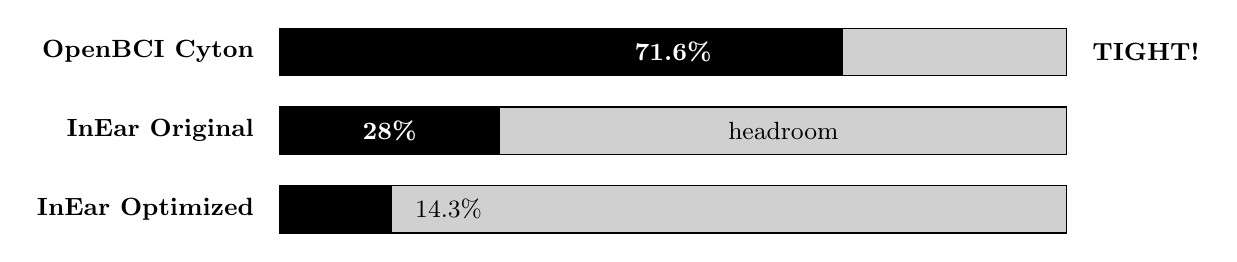
\begin{tikzpicture}[x=0.2cm, y=1cm]
    % OpenBCI
    \node[anchor=east] at (-1, 2) {\small\textbf{OpenBCI Cyton}};
    \fill[black] (0, 1.7) rectangle (35.8, 2.3);
    \fill[lightgray] (35.8, 1.7) rectangle (50, 2.3);
    \draw (0, 1.7) rectangle (50, 2.3);
    \node at (25, 2) {\small\color{white}\textbf{71.6\%}};
    \node[anchor=west] at (51, 2) {\small\textbf{TIGHT!}};
    
    % InEar Original
    \node[anchor=east] at (-1, 1) {\small\textbf{InEar Original}};
    \fill[black] (0, 0.7) rectangle (14, 1.3);
    \fill[lightgray] (14, 0.7) rectangle (50, 1.3);
    \draw (0, 0.7) rectangle (50, 1.3);
    \node at (7, 1) {\small\color{white}\textbf{28\%}};
    \node at (32, 1) {\small headroom};
    
    % InEar Optimized
    \node[anchor=east] at (-1, 0) {\small\textbf{InEar Optimized}};
    \fill[black] (0, -0.3) rectangle (7.15, 0.3);
    \fill[lightgray] (7.15, -0.3) rectangle (50, 0.3);
    \draw (0, -0.3) rectangle (50, 0.3);
    \node[anchor=west] at (8, 0) {\small 14.3\%};
\end{tikzpicture}
\caption{Bandwidth utilization comparison (bar chart). Each bar represents the percentage of the serial link capacity used.}
\label{fig:headroom}
\end{figure}

\subsection{Where The Bytes Go (Original)}

\begin{table}[H]
\centering
\begin{tabular}{|l|R{2cm}|R{1.5cm}|}
\hline
\textbf{Component} & \textbf{B/s} & \textbf{\% of total} \\\hline
EEG (brain signals) & 15,000 & 26.8\% \\
\textbf{PPG (heart pulse)} & \textbf{18,000} & \textbf{32.1\%} \\
Accelerometer & 6,000 & 10.7\% \\
Temp + Battery & 4,000 & 7.1\% \\
Sync & 2,000 & 3.6\% \\
Overhead (hdr+ts+mkr+ctr+chk+ftr) & 11,000 & 19.6\% \\
\hline
\textbf{Total} & \textbf{56,000} & \\
\hline
\end{tabular}
\caption{Byte budget breakdown --- InEar Original. PPG alone = 18,000\,B/s = 32\% of all traffic!}
\end{table}

\subsection{Where The Bytes Go (Optimized)}

\begin{table}[H]
\centering
\begin{tabular}{|l|R{2cm}|R{1.5cm}|}
\hline
\textbf{Component} & \textbf{B/s} & \textbf{\% of total} \\\hline
EEG (every packet) & 15,000 & 52.6\% \\
Accel (every 4th) & 1,500 & 5.3\% \\
PPG (every 10th) & 1,800 & 6.3\% \\
Health (every 100th) & 40 & 0.1\% \\
Headers/footers & ${\sim}$10,160 & 35.6\% \\
\hline
\textbf{Total} & $\mathbf{{\sim}28{,}500}$ & \\
\hline
\end{tabular}
\caption{Byte budget breakdown --- InEar Optimized. \textbf{Savings vs.\ original: ${\sim}$49\%}}
\end{table}

% =============================================================================
\section{How The Stream Looks Over Time}
\label{sec:stream-behavior}

\subsection{How Packets Flow}

\begin{lstlisting}[style=diagram, caption={Packet timing comparison}]
OpenBCI Cyton (250 Hz, uniform):
 --[33B]---[33B]---[33B]---[33B]---[33B]---  (4 ms apart)

InEar Original (1000 Hz, uniform):
 -[56]-[56]-[56]-[56]-[56]-[56]-[56]-[56]-  (1 ms apart, same every time)

InEar Optimized (1000 Hz, variable):
 -[26]-[26]-[26]-[32]-[26]-[26]-[26]-[32]-[26]-[50]-[26]-[26]-
   ^         ^              ^          ^
   |         |              |          +- EEG + accel + PPG (every 20th)
   |         |              +- EEG + accel (every 4th)
   |         +- EEG + accel (every 4th)
   +- EEG only (most common - small and fast!)
\end{lstlisting}

\subsection{What 1 Second of Data Looks Like}

In one second (1000 packets), the optimized protocol sends:

\begin{table}[H]
\centering
\begin{tabular}{|l|r|r|r|}
\hline
\textbf{Packet Type} & \textbf{Size} & \textbf{Count/sec} & \textbf{\% of packets} \\\hline
\hline
EEG-only & 26\,B & 749 & 74.9\% \\
EEG + Accel & 32\,B & 200 & 20.0\% \\
EEG + PPG & 44\,B & 40 & 4.0\% \\
EEG + Accel + PPG & 50\,B & 9 & 0.9\% \\
EEG + Health & 30\,B & ${\sim}$1 & 0.1\% \\
EEG + Full Sync & 54\,B & 1 & 0.1\% \\
\hline
\textbf{Total} & & \textbf{1000} & \\
\hline
\end{tabular}
\caption{Packet type distribution. 75\% of packets are the small 26-byte EEG-only type.}
\end{table}

\subsection{What Happens When Data Is Missing?}

When the optimized protocol sends an EEG-only packet (no accel), the receiver doesn't show a gap --- it just \textbf{holds the last value}:

\begin{lstlisting}[style=diagram, caption={Sample-and-hold behavior for multi-rate sensors}]
Time:   1ms   2ms   3ms   4ms   5ms   6ms   7ms   8ms
EEG:    new   new   new   new   new   new   new   new   (every packet)
Accel:  new   held  held  NEW   held  held  held  NEW   (every 4th)
PPG:    new   held  held  held  held  held  held  held  (every 10th)
\end{lstlisting}

Accel hasn't changed in 4\,ms. PPG hasn't changed in 10\,ms. No information lost.

% =============================================================================
\section{Original vs.\ Optimized --- Tradeoffs}
\label{sec:tradeoff-matrix}

\begin{table}[H]
\centering
\small
\begin{tabular}{|l|>{\raggedright\arraybackslash}p{3.5cm}|>{\raggedright\arraybackslash}p{3.5cm}|>{\raggedright\arraybackslash}p{3.8cm}|}
\hline
\textbf{Dimension} & \textbf{InEar Original} & \textbf{InEar Optimized} & \textbf{Winner} \\\hline
Bandwidth & 56\,KB/s & ${\sim}$28.5\,KB/s & \ding{51} Optimized (49\% less) \\
Latency & 280\,$\mu$s wire & 130--270\,$\mu$s wire & \ding{51} Optimized \\
Integrity & XOR checksum & XOR checksum & = Tie \\
Parser Complexity & Simple: fixed offsets & Complex: 14 types & \ding{51} Original \\
Firmware Complexity & Simple: fill 56\,B & Moderate: variable & \ding{51} Original \\
Jitter Robustness & Excellent: uniform & Good: variable sizes & \ding{51} Original \\
Packet Loss Robustness & Good: self-contained & Moderate: stale data & \ding{51} Original \\
Headroom & 72\% free & 86\% free & \ding{51} Optimized \\
Memory Efficiency & All bytes used & Zero overhead & = Tie \\
Extensibility & Fixed layout & New packet type needed & \ding{51} Original \\
\hline
\end{tabular}
\caption{Head-to-head trade-off comparison}
\label{tab:tradeoff}
\end{table}

% =============================================================================
\section{All The Optimization Ideas (28 Tactics)}
\label{sec:taxonomy}

28 optimization ideas in 7 categories, starting from the 56-byte fixed protocol.

\subsection{Category 1: Bandwidth Optimization}
\textit{Fewer bytes on the wire}

\begin{table}[H]
\centering
\small
\begin{tabularx}{\textwidth}{|c|l|X|}
\hline
\textbf{ID} & \textbf{Tactic} & \textbf{Description} \\\hline
\tactic{1A} \implemented & Multi-rate aux sampling & Send aux sensors only at their Nyquist rate \\
\tactic{1B} & Delta encoding for EEG & Send differences instead of absolute values \\
\tactic{1C} & Variable-width integers & Small values use fewer bytes \\
\tactic{1E} & PPG to 24-bit & PPG ADCs are 18--20\,bit; 24-bit is plenty \\
\tactic{1F} & Smaller header & Reduce or compress header fields \\
\tactic{1G} & Multi-sample batching & Pack N samples per packet, amortize overhead \\
\hline
\end{tabularx}
\caption{Category 1: Bandwidth optimization tactics}
\end{table}

\subsection{Category 2: Latency Optimization}
\textit{Faster ADC-to-screen time}

\begin{table}[H]
\centering
\small
\begin{tabularx}{\textwidth}{|c|l|X|}
\hline
\textbf{ID} & \textbf{Tactic} & \textbf{Description} \\\hline
\tactic{2A} & Reduce packet size & Smaller packet = faster on wire (covered by Cat.~1) \\
\tactic{2B} & Increase baud rate & Teensy~4.1 supports up to 6\,Mbaud \\
\tactic{2C} & USB flush optimization & Use \texttt{Serial.send\_now()} for immediate transfer \\
\tactic{2D} & DMA SPI$\to$UART pipeline & Hardware transfers without CPU involvement \\
\hline
\end{tabularx}
\caption{Category 2: Latency optimization tactics}
\end{table}

\subsection{Category 3: Integrity Optimization}
\textit{Catching errors before they corrupt data}

\begin{table}[H]
\centering
\small
\begin{tabularx}{\textwidth}{|c|l|X|}
\hline
\textbf{ID} & \textbf{Tactic} & \textbf{Description} \\\hline
\tactic{3A} & CRC-8 or CRC-16 & Better error detection than XOR checksum \\
\tactic{3B} & Forward Error Correction & Correct errors without retransmission (Hamming/RS) \\
\tactic{3C} & Retransmission (ARQ) & Receiver requests re-send of bad packets \\
\tactic{3D} & Longer sync pattern & 3--4 byte sync for fewer false positives \\
\tactic{3E} & Explicit length field & Self-describing packets, forward-compatible \\
\hline
\end{tabularx}
\caption{Category 3: Integrity optimization tactics}
\end{table}

\subsection{Category 4: Parser/CPU Optimization}
\textit{Faster host-side parsing}

\begin{table}[H]
\centering
\small
\begin{tabularx}{\textwidth}{|c|l|X|}
\hline
\textbf{ID} & \textbf{Tactic} & \textbf{Description} \\\hline
\tactic{4A} & Ring buffer & Replace \texttt{std::deque} with fixed circular buffer \\
\tactic{4B} & Zero-copy parsing & Parse directly from buffer, skip memcpy \\
\tactic{4C} & SIMD byte conversion & Parallel 24-bit $\to$ 32-bit conversion \\
\tactic{4D} & Remove \texttt{std::chrono} & Avoid syscalls during packet parsing \\
\tactic{4E} & Batch \texttt{addToBuffer()} & Fewer lock acquisitions in Open Ephys \\
\hline
\end{tabularx}
\caption{Category 4: Parser/CPU optimization tactics}
\end{table}

\subsection{Category 5: Firmware CPU Optimization}
\textit{Less Teensy CPU usage}

\begin{table}[H]
\centering
\small
\begin{tabularx}{\textwidth}{|c|l|X|}
\hline
\textbf{ID} & \textbf{Tactic} & \textbf{Description} \\\hline
\tactic{5A} & Precomputed templates & Pre-fill headers, only overwrite data fields \\
\tactic{5B} & Packet type lookup table & Replace modulo operations with array lookup \\
\tactic{5C} & ISR-based assembly & Build packets in interrupt handler \\
\hline
\end{tabularx}
\caption{Category 5: Firmware CPU optimization tactics}
\end{table}

\subsection{Category 6: Robustness Optimization}
\textit{Reliable connections, no data loss}

\begin{table}[H]
\centering
\small
\begin{tabularx}{\textwidth}{|c|l|X|}
\hline
\textbf{ID} & \textbf{Tactic} & \textbf{Description} \\\hline
\tactic{6A} & Heartbeat/watchdog & Detect disconnections immediately \\
\tactic{6B} & Connection handshake & Verify firmware version before streaming \\
\tactic{6C} & Configurable sample rate & Host can change rate (250/500/1000/2000\,Hz) \\
\tactic{6D} & Per-channel gain control & Host can set ADS1299 gain per channel \\
\hline
\end{tabularx}
\caption{Category 6: Robustness optimization tactics}
\end{table}

\subsection{Category 7: Data Quality Optimization}
\textit{Better data for research}

\begin{table}[H]
\centering
\small
\begin{tabularx}{\textwidth}{|c|l|X|}
\hline
\textbf{ID} & \textbf{Tactic} & \textbf{Description} \\\hline
\tactic{7A} & Hardware clock sync & Sub-microsecond timing via host$\leftrightarrow$device sync \\
\tactic{7B} & Impedance measurement & Report electrode impedance in packets \\
\tactic{7C} & Higher sample rate & ADS1299 supports up to 16\,kHz \\
\hline
\end{tabularx}
\caption{Category 7: Data quality optimization tactics}
\end{table}

% =============================================================================
\section{Detailed Notes On Each Tactic}
\label{sec:tactic-details}

\subsection{Category 1 --- Bandwidth}

% --- 1A ---
\subsubsection{1A --- Multi-Rate Auxiliary Sampling \implemented}

Send each sensor at a rate matching how fast it actually changes (Nyquist rate), not all at 1000\,Hz.

\begin{table}[H]
\centering
\begin{tabular}{|l|r|r|r|r|}
\hline
\textbf{Sensor} & \textbf{BW of Interest} & \textbf{Nyquist Min} & \textbf{Send Rate} & \textbf{Oversampling} \\\hline
\hline
EEG & 0.1--300\,Hz & 600\,Hz & 1000\,Hz & $1.67\times$ \\
Accelerometer & 0--100\,Hz & 200\,Hz & 250\,Hz & $1.25\times$ \\
PPG & 0.5--25\,Hz & 50\,Hz & 100\,Hz & $2\times$ \\
Temperature & ${\sim}$0\,Hz (DC) & ${\sim}$1\,Hz & 10\,Hz & $10\times$ \\
\hline
\end{tabular}
\caption{Nyquist justification for multi-rate scheduling}
\end{table}

\textbf{Why}: Temperature changes over seconds. Sending it $1000\times$/sec = same reading every time.

\textbf{Trade-off}: Parser goes from 1 packet type to 14 (7 base $\times$ 2 with marker). Receiver needs sample-and-hold. Lost PPG packet = stale for 10\,ms not 1\,ms.

\textbf{Impact}: Saves ${\sim}$49\% bandwidth ($56{,}000 \to {\sim}28{,}500$\,B/s).

% --- 1B ---
\subsubsection{1B --- Delta Encoding for EEG}

Send differences between consecutive samples instead of absolute values. At 1\,kHz, EEG deltas fit in 8--12 bits vs.\ 24.

\begin{lstlisting}[style=diagram, caption={Delta encoding example}]
Absolute:  sample1 = 123456    -> 3 bytes (24-bit)
           sample2 = 123489    -> 3 bytes (24-bit)
           sample3 = 123501    -> 3 bytes (24-bit)

Delta:     sample1 = 123456    -> 3 bytes (24-bit, keyframe)
           d2 = +33            -> 1 byte  (8-bit delta)
           d3 = +12            -> 1 byte  (8-bit delta)

Savings: 9 bytes -> 5 bytes for 3 samples (44%)
\end{lstlisting}

\textbf{Note to self:} Losing one packet corrupts everything until the next keyframe. Need periodic absolute keyframes (e.g., every 100 samples) and gap detection via sequence numbers. Potential savings: 40--60\% for EEG.

% --- 1C ---
\subsubsection{1C --- Variable-Width Integers (VarInt)}

Small values use fewer bytes (like Protocol Buffers).

\textbf{Trade-off}:
\begin{itemize}
    \item[\ding{55}] Packets have \textbf{unpredictable size} --- parser can't jump to fixed offsets
    \item[\ding{55}] Bit-level parsing is expensive
    \item[\ding{55}] Cannot pre-validate packet size
    \item[\ding{51}] Average savings of ${\sim}$30\% combined with delta encoding
\end{itemize}

\textbf{Verdict}: High complexity, moderate savings. Better for file formats than real-time streams.

% --- 1E ---
\subsubsection{1E --- PPG to 24-bit (from 48-bit) \freewin}

PPG is 48-bit (6 bytes/channel) but the MAX30105 ADC is 18-bit. 24-bit (3 bytes) is enough.

\begin{align}
\text{Current:} \quad & 3 \text{ channels} \times 6 \text{\,B} = 18 \text{\,B/sample} \nonumber\\
\text{Proposed:} \quad & 3 \text{ channels} \times 3 \text{\,B} = 9 \text{\,B/sample} \nonumber\\
\text{Savings:} \quad & 9 \text{\,B per PPG packet} \nonumber
\end{align}

Firmware uses \texttt{packInt48BE()}, top 3 bytes always zero. 24-bit = 16.7M levels for ${\sim}$18 bits of data. Sufficient.

\textbf{Trade-off}: None. Free win.

% --- 1F ---
\subsubsection{1F --- Smaller Header/Footer}

Current: 2-byte header (\hexval{A5}\,\hexval{5A}) + 2-byte footer (\hexval{C0}\,\hexval{C0}) = 4\,bytes/packet.

\textbf{False sync math}: With a 2-byte header, false sync probability is $1/65{,}536$. With 1-byte: $1/256$ --- $256\times$ more likely.

\textbf{Verdict}: Saves 1--3\,B/pkt, makes resyncing harder. Not worth it.

% --- 1G ---
\subsubsection{1G --- Multi-Sample Batching}

Pack $N$ samples per packet, share header/footer/checksum cost.

\begin{align}
\text{Current (1/pkt):} \quad & 3 \times 26 = 78 \text{\,B for 3 samples, 33\,B overhead (42\%)} \nonumber\\
\text{Batched (3/pkt):} \quad & 8 + 3 \times 15 + 3 = 56 \text{\,B for 3 samples, 11\,B overhead (20\%)} \nonumber
\end{align}

\textbf{Trade-off}:
\begin{itemize}
    \item[\ding{55}] Latency increases by $N\times$ (at 1\,kHz with $N=4$: 4\,ms instead of 1\,ms)
    \item[\ding{55}] Losing one packet loses $N$ samples
    \item[\ding{51}] At $N=4$, overhead drops from 42\% to 17\%
\end{itemize}

\textbf{Verdict}: Bad for real-time neurofeedback. OK for recording.

\subsection{Category 2 --- Latency}

% --- 2A ---
\subsubsection{2A --- Reduce Packet Size}

Side effect of Category 1. Smaller packet = less wire time.

\begin{align}
\text{Original (56\,B):} \quad & 56 \times 10 / 2{,}000{,}000 = 280\,\mu\text{s} \nonumber\\
\text{Optimized (26\,B):} \quad & 26 \times 10 / 2{,}000{,}000 = 130\,\mu\text{s} \;\;(54\% \text{ faster}) \nonumber
\end{align}

% --- 2B ---
\subsubsection{2B --- Increase Baud Rate}

Teensy~4.1 supports up to 6\,Mbaud. Currently at 2\,Mbaud.

\begin{table}[H]
\centering
\begin{tabular}{|r|r|r|r|}
\hline
\textbf{Baud Rate} & \textbf{Max B/s} & \textbf{Wire time (56\,B)} & \textbf{Wire time (26\,B)} \\\hline
\hline
2,000,000 & 200,000 & 280\,$\mu$s & 130\,$\mu$s \\
3,000,000 & 300,000 & 187\,$\mu$s & 87\,$\mu$s \\
4,000,000 & 400,000 & 140\,$\mu$s & 65\,$\mu$s \\
6,000,000 & 600,000 & 93\,$\mu$s & 43\,$\mu$s \\
\hline
\end{tabular}
\caption{Wire time at various baud rates}
\end{table}

{\sloppy \textbf{Trade-off}: Higher bit error rate, USB-serial IC may not support it, cable quality matters above 3\,Mbaud.
Low priority --- 130\,$\mu$s is small vs.\ 1\,ms sample period.\par}

% --- 2C ---
\subsubsection{2C --- USB Flush Optimization}

Call \texttt{Serial.send\_now()} to flush USB immediately instead of waiting for the ${\sim}$1\,ms default buffer interval.

\begin{lstlisting}[style=cpp, caption={USB flush optimization}]
Serial.write(packet, len);
Serial.send_now();  // Force immediate USB transfer
// USB packet sent on next USB frame (~125 us for USB 2.0 HS)
\end{lstlisting}

\textbf{Verdict}: One line of code. Removes up to 1\,ms latency. Not implemented.

% --- 2D ---
\subsubsection{\texorpdfstring{2D --- DMA SPI\textrightarrow UART Pipeline}{2D --- DMA SPI to UART Pipeline}}

DMA hardware transfers data from ADS1299 SPI to UART without CPU.

\begin{lstlisting}[style=diagram, caption={CPU-mediated vs.\ DMA data flow}]
Current:  ADS1299 --SPI--> [CPU reads] --> [CPU builds] --> [CPU writes UART]
DMA:      ADS1299 --SPI--> [DMA->RAM]  --> [CPU builds] --> [DMA->UART]
                            ^ HW only ^                      ^ HW only ^
\end{lstlisting}

\textbf{Verdict}: High effort, high reward. Only useful if Teensy needs CPU for other tasks.

\subsection{Category 3 --- Integrity}

% --- 3A ---
\subsubsection{3A --- CRC-8 Instead of XOR \freewin}

Same 1-byte cost as XOR, much better error detection:

\begin{table}[H]
\centering
\begin{tabular}{|l|c|c|}
\hline
\textbf{Error Type} & \textbf{XOR} & \textbf{CRC-8} \\\hline
\hline
Single-bit errors & 100\% & 100\% \\
2-bit errors & 100\% & 100\% \\
Odd \# of bit errors & 100\% & 100\% \\
Even \# of bit errors & \textbf{0\%!!} & 99.6\% \\
Burst errors ($\leq$8 bit) & ${\sim}$50\% & 100\% \\
Random errors & ${\sim}$50\% & 99.6\% \\
\hline
\end{tabular}
\caption{Error detection: XOR vs.\ CRC-8}
\end{table}

Needs a 256-byte lookup table and one lookup per byte. 56,000 lookups/sec on a 600\,MHz Teensy = negligible.

% --- 3B ---
\subsubsection{3B --- Forward Error Correction (FEC)}

Add redundancy bytes to correct errors without retransmission (Hamming, Reed-Solomon).

\textbf{Verdict}: Overkill for wired USB. USB~2.0 has hardware CRC16. Only relevant for lossy links (e.g.\ Gazell).

% --- 3C ---
\subsubsection{3C --- Retransmission (ARQ)}

Receiver sends NACK on bad packets; firmware re-sends.

\textbf{Trade-off}: 2--3\,ms latency per retry, needs bidirectional protocol and TX buffer on Teensy. Near-zero USB loss rate = not needed.

% --- 3D ---
\subsubsection{3D --- Longer Sync Pattern}

Use 3--4 byte sync instead of current 2-byte \hexval{A5}\,\hexval{5A}.

\begin{align}
\text{2-byte:} \quad & P(\text{false sync}) = 1/2^{16} = 1/65{,}536 \nonumber\\
\text{3-byte:} \quad & P(\text{false sync}) = 1/2^{24} = 1/16{,}777{,}216 \nonumber\\
\text{4-byte:} \quad & P(\text{false sync}) = 1/2^{32} \approx 1/4.3 \times 10^9 \nonumber
\end{align}

\textbf{Verdict}: Current 2-byte + checksum is sufficient.

% --- 3E ---
\subsubsection{3E --- Explicit Length Field}

Add a 1-byte length field so the parser knows the exact packet size before reading.

\textbf{Trade-off}: +1\,byte/packet (1,000\,B/s). Host can skip unknown packet types without a lookup table.

\textbf{Verdict}: Good trade-off. Worth doing in any evolving protocol.

\subsection{Category 4 --- Parser/CPU (Host Side)}

% --- 4A ---
\subsubsection{4A --- Ring Buffer Instead of \texttt{std::deque} \freewin}

Current parser uses \texttt{std::deque<uint8\_t>}. Each \texttt{push\_back()}/\texttt{pop\_front()} may allocate heap. At 28,500\,B/s = up to 28,500 allocs/sec, bad cache locality.

Fixed 16\,KB circular buffer removes all allocations:

\begin{lstlisting}[style=cpp, caption={Ring buffer implementation sketch}]
class RingBuffer {
    uint8_t buffer[16384];  // 16 KB, power of 2
    size_t head = 0, tail = 0;
public:
    void push(const uint8_t* data, size_t len) {
        for (size_t i = 0; i < len; i++)
            buffer[(tail++) & 0x3FFF] = data[i];
    }
    uint8_t operator[](size_t i) const {
        return buffer[(head + i) & 0x3FFF];
    }
    void consume(size_t n) { head += n; }
    size_t available() const { return tail - head; }
};
\end{lstlisting}

No allocations in hot path. Better cache. Same behavior.

% --- 4B ---
\subsubsection{4B --- Zero-Copy Parsing}

Parse directly from ring buffer, skip the copy to a temp struct.

\textbf{Trade-off}: Must handle wrap-around mid-packet. Saves one memcpy/packet (56\,B $\times$ 1000/sec = 56\,KB/s eliminated). Best combined with 4A.

% --- 4C ---
\subsubsection{4C --- SIMD Byte Conversion}

SSE/AVX (x86) or NEON (ARM) for parallel 24-bit BE $\to$ 32-bit signed conversion.

\textbf{Verdict}: Only 5 channels. Sequential code takes nanoseconds. Not worth platform-specific code.

% --- 4D ---
\subsubsection{4D --- Remove \texttt{std::chrono} from Hot Path \freewin}

Parser calls \texttt{std::chrono::steady\_clock::now()} every \texttt{updateBuffer()} for bandwidth monitoring. On Windows = kernel syscall.

\textbf{Fix}: Use packet counter (\texttt{if (count \% 5000 == 0)}).

\textbf{Effort}: ${\sim}$10 min, 3--4 lines.

% --- 4E ---
\subsubsection{4E --- Batch \texttt{addToBuffer()} Calls}

1 call/packet = 1000 lock cycles/sec. Batch $N$ samples = $1000/N$ locks.

\textbf{Trade-off}: Up to $N$\,ms extra latency. Good for throughput, bad for real-time.

\subsection{Category 5 --- Firmware CPU (Teensy Side)}

% --- 5A ---
\subsubsection{5A --- Precomputed Packet Templates}

Pre-fill static fields (header, footer, type) at startup into 7 templates. In ISR: \texttt{memcpy} template, overwrite dynamic fields.

\textbf{Trade-off}: $7 \times 55 = 385$\,bytes RAM. Teensy has 1\,MB. Negligible.

% --- 5B ---
\subsubsection{5B --- Packet Type Lookup Table \freewin}

Replace cascading modulo with a precomputed 1000-entry array.

\begin{lstlisting}[style=cpp, caption={Packet type lookup table}]
// Current: 5 modulo operations + 5 branches
uint8_t getPacketType(uint32_t n) {
    if (n % 1000 == 0) return 0x06;
    if (n % 100 == 0)  return 0x04;
    if (n % 20 == 0)   return 0x03;
    if (n % 10 == 0)   return 0x02;
    if (n % 4 == 0)    return 0x01;
    return 0x00;
}

// Proposed: 1 modulo + 1 array read
static uint8_t typeTable[1000];  // precomputed at startup
uint8_t type = typeTable[sampleNum % 1000];
\end{lstlisting}

Uses 1000\,bytes of RAM. Teensy has 1\,MB. \textbf{Free win}.

% --- 5C ---
\subsubsection{5C --- ISR-Based Packet Assembly}

Build packets in IntervalTimer ISR for deterministic timing.

\textbf{Status}: Already implemented. Firmware builds and sends in ISR callback.

\subsection{Category 6 --- Robustness}

% --- 6A ---
\subsubsection{6A --- Heartbeat / Watchdog}

Firmware sends ``I'm alive'' packet every ${\sim}$1 sec. No heartbeat for $N$ seconds = connection dead.

\begin{lstlisting}[style=diagram, caption={Heartbeat disconnect detection}]
Normal:   Host <--- [Data] [Data] [HB] [Data] --- Teensy

Failure:  Host <--- [Data] [Data]             --- (cable yanked!)
          ...3 seconds, no heartbeat...
          HOST: CONNECTION LOST -> show error, clean up
\end{lstlisting}

\textbf{Verdict}: ${\sim}$10\,B/s overhead. Easy to add.

% --- 6B ---
\subsubsection{6B --- Connection Handshake}

Startup: \texttt{HELLO} $\to$ Device Info $\to$ \texttt{START} $\to$ streaming $\to$ \texttt{STOP} $\to$ \texttt{OK}.

Auto-detects firmware version, channel count, sample rate. Prevents mismatch.

\textbf{Trade-off}: +${\sim}$100\,ms startup. Negligible.

% --- 6C ---
\subsubsection{6C --- Configurable Sample Rate}

Host sets Teensy sample rate at runtime.

\begin{table}[H]
\centering
\begin{tabular}{|r|l|}
\hline
\textbf{Rate} & \textbf{Use Case} \\\hline
\hline
250\,Hz & Low power, clinical EEG \\
500\,Hz & Balanced research EEG \\
1000\,Hz & High-frequency EEG (current default) \\
2000\,Hz & Fast neural events \\
4000\,Hz & EMG, specialized \\
\hline
\end{tabular}
\caption{ADS1299 configurable sample rates}
\end{table}

\textbf{Verdict}: Useful. Pairs with handshake (6B). Moderate effort.

% --- 6D ---
\subsubsection{6D --- Per-Channel Gain Control}

Set ADS1299 PGA gain per channel at runtime. Gains: $1\times$, $2\times$, $4\times$, $6\times$, $8\times$, $12\times$, $24\times$.

\textbf{Use case}: Channels 1--4 at $24\times$ (EEG) and channel 5 at $1\times$ (EMG for jaw clench detection).

\subsection{Category 7 --- Data Quality}

% --- 7A ---
\subsubsection{7A --- Hardware Clock Synchronization}

Sync Teensy crystal with host clock. Without it: ${\sim}$50\,ppm drift $\rightarrow$ 180\,ms off after 1 hour.

\textbf{Method}: Periodic NTP-style time exchange ($T_1, T_2, T_3, T_4$):
\[
\text{Offset} = \frac{(T_2 - T_1) + (T_3 - T_4)}{2}, \qquad
\text{RTT} = (T_4 - T_1) - (T_3 - T_2)
\]

After correction: ${\sim}100\,\mu$s accuracy. Required for multi-device setups.

% --- 7B ---
\subsubsection{7B --- Impedance Measurement}

Use ADS1299's built-in impedance mode to check electrode contact quality.

\begin{table}[H]
\centering
\begin{tabular}{|r|l|l|}
\hline
\textbf{Impedance} & \textbf{Quality} & \textbf{Interpretation} \\\hline
\hline
$< 10$\,k$\Omega$ & \ding{51} Good & Gel electrodes, well-placed \\
$10$--$50$\,k$\Omega$ & $\triangle$ Acceptable & Dry electrodes, may work \\
$> 50$\,k$\Omega$ & \ding{55} Poor & Needs adjustment \\
$> 1$\,M$\Omega$ & \ding{55} None & No electrode detected \\
\hline
\end{tabular}
\caption{Electrode impedance quality thresholds}
\end{table}

\textbf{Verdict}: Useful for research. Setup-time only, not during streaming.

% --- 7C ---
\subsubsection{7C --- Higher Sample Rate}

ADS1299 supports up to 16\,kHz. Bandwidth implications:

\begin{table}[H]
\centering
\begin{tabular}{|r|r|r|l|}
\hline
\textbf{Rate} & \textbf{B/s (opt)} & \textbf{Utilization} & \textbf{Status} \\\hline
\hline
250\,Hz & ${\sim}$7,125 & 3.6\% & OK \\
500\,Hz & ${\sim}$14,250 & 7.1\% & OK \\
1,000\,Hz & ${\sim}$28,500 & 14.3\% & Current \\
2,000\,Hz & ${\sim}$57,000 & 28.5\% & OK \\
4,000\,Hz & ${\sim}$114,000 & 57.0\% & Tight \\
8,000\,Hz & ${\sim}$228,000 & 114\% & \textbf{Exceeds 2\,Mbaud!} \\
16,000\,Hz & ${\sim}$456,000 & 228\% & \textbf{Need 6\,Mbaud+} \\
\hline
\end{tabular}
\caption{Sample rate vs.\ bandwidth utilization}
\end{table}

Current protocol supports up to ${\sim}$4000\,Hz within the 2\,Mbaud link budget.

% =============================================================================
\section{The Big Trade-Off Table}
\label{sec:full-matrix}

\metricdown\ = good (reduces/improves), \metricup\ = bad (increases/worsens), \metriceq\ = doesn't matter.

{
\setlength{\tabcolsep}{3pt}
\tiny
\begin{longtable}{|l|C{1.5cm}|C{1.3cm}|C{1.3cm}|C{1.3cm}|C{1.3cm}|C{1.7cm}|C{1.5cm}|}
\caption{Full 28-tactic trade-off matrix} \label{tab:full-matrix} \\
\hline
\textbf{Tactic} & \textbf{BW} & \textbf{Latency} & \textbf{Integrity} & \textbf{Parser} & \textbf{FW CPU} & \textbf{Complex.} & \textbf{Robust.} \\\hline
\endfirsthead
\hline
\textbf{Tactic} & \textbf{BW} & \textbf{Latency} & \textbf{Integrity} & \textbf{Parser} & \textbf{FW CPU} & \textbf{Complex.} & \textbf{Robust.} \\\hline
\endhead
\hline
\endfoot

\tactic{1A} Multi-rate &
\metricdown\metricdown\ 49\% &
\metricdown\ smaller &
\metriceq &
\metricup\metricup\ state mach. &
\metricup\ modulo &
\metricup\metricup\ 14 types &
\metricdown\ stale risk \\

\tactic{1B} Delta enc. &
\metricdown\metricdown\metricdown\ 60\% &
\metricdown\ smaller &
\metricdown\metricdown\metricdown\ propagates &
\metricup\metricup\ accum. &
\metricup\ delta math &
\metricup\metricup\metricup\ keyframes &
\metricdown\metricdown\metricdown\ corrupts \\

\tactic{1C} VarInt &
\metricdown\metricdown\ 30\% &
\metricdown\ smaller &
\metricdown\ no pre-val &
\metricup\metricup\metricup\ bit parse &
\metricup\ encoding &
\metricup\metricup\metricup\ no fixed &
\metricdown\metricdown\ unpredict. \\

\tactic{1E} PPG 24-bit &
\metricdown\ 9\,B/PPG &
\metricdown\ 9\,B less &
\metriceq &
\metricdown\ reuse parser &
\metricdown\ simpler &
\metricdown\ fewer widths &
\metriceq \\

\tactic{1F} Sm.\ header &
\metricdown\ 2--4\,B &
\metricdown\ slight &
\metricdown\ less resync &
\metriceq &
\metricdown\ fewer B &
\metricup\ tighter &
\metricdown\ less recov. \\

\tactic{1G} Batch $N$ &
\metricdown\metricdown\ amortize &
\metricup\metricup\ $N\times$1\,ms &
\metricup\ lose $N$ &
\metricup\ unpack &
\metricup\ buffer &
\metricup\metricup\ edge cases &
\metricdown\metricdown\ more loss \\

\tactic{2A} Reduce size &
\metricdown\ (via Cat 1) &
\metricdown\ fewer bits &
\metriceq &
\metriceq &
\metriceq &
\metriceq &
\metriceq \\

\tactic{2B} Higher baud &
\metriceq &
\metricdown\ faster wire &
\metricdown\ higher BER &
\metriceq &
\metriceq\ config &
\metriceq\ config &
\metricdown\ bit errors \\

\tactic{2C} send\_now() &
\metriceq &
\metricdown\ 0.5\,ms &
\metriceq &
\metriceq &
\metricup\ USB IRQs &
\metricup\ ISR timing &
\metriceq \\

\tactic{2D} DMA &
\metriceq &
\metricdown\metricdown\ no CPU &
\metriceq &
\metriceq &
\metricdown\metricdown\ freed &
\metricup\metricup\ setup &
\metricup\ HW xfer \\

\tactic{3A} CRC-8 &
\metriceq\ same &
\metriceq &
\metricdown\metricdown\ 99.6\% &
\metricup\ table lkup &
\metricup\ table lkup &
\metricup\ 256\,B table &
\metricup\ fewer undet. \\

\tactic{3B} FEC &
\metricup\metricup\ 20--50\% &
\metricup\ enc/dec &
\metricdown\metricdown\metricdown\ corrects &
\metricup\metricup\metricup\ decode &
\metricup\metricup\metricup\ encode &
\metricup\metricup\metricup\ overkill &
\metricup\metricup\ corrected \\

\tactic{3C} Retransmit &
\metricup\ NACK &
\metricup\metricup\ round-trip &
\metricdown\metricdown\ guaranteed &
\metricup\metricup\ reorder &
\metricup\metricup\ TX buf &
\metricup\metricup\metricup\ bidir. &
\metricup\metricup\metricup\ no loss \\

\tactic{3D} Longer sync &
\metricup\ +1--2\,B &
\metriceq &
\metricup\ lower false &
\metriceq &
\metriceq &
\metriceq &
\metricup\ reliable \\

\tactic{3E} Length field &
\metricup\ +1\,B &
\metriceq &
\metricup\ validate &
\metricdown\ no LUT &
\metricup\ +1 byte &
\metricdown\ fwd-compat &
\metricup\ new types \\

\tactic{4A} Ring buffer &
\metriceq &
\metricdown\ alloc jitter &
\metriceq &
\metricdown\metricdown\ no heap &
\metriceq &
\metricup\ wraparound &
\metricup\ determin. \\

\tactic{4B} Zero-copy &
\metriceq &
\metricdown\ less memcpy &
\metriceq &
\metricdown\ no copy &
\metriceq &
\metricup\ wrap parse &
\metriceq \\

\tactic{4C} SIMD &
\metriceq &
\metricdown\ faster cvt &
\metriceq &
\metricdown\ parallel &
\metriceq &
\metricup\metricup\ platform &
\metriceq \\

\tactic{4D} Rm.\ chrono &
\metriceq &
\metricdown\ fewer sys &
\metriceq &
\metricdown\ no syscall &
\metriceq &
\metricdown\ simpler &
\metricup\ determin. \\

\tactic{4E} Batch addTo &
\metriceq &
\metricup\ batch delay &
\metriceq &
\metricdown\ fewer locks &
\metriceq &
\metricup\ batch code &
\metriceq \\

\tactic{5A} Templates &
\metriceq &
\metriceq &
\metriceq &
\metriceq &
\metricdown\ fewer wr. &
\metricdown\ cleaner &
\metriceq \\

\tactic{5B} Type LUT &
\metriceq &
\metriceq &
\metriceq &
\metriceq &
\metricdown\ 1 vs 5 mod &
\metricdown\ simpler &
\metriceq \\

\tactic{5C} ISR assembly &
\metriceq &
\metricdown\ no loop &
\metriceq &
\metriceq &
\metricup\ longer ISR &
\metricup\ overrun &
\metricup\ determin. \\

\tactic{6A} Heartbeat &
\metricup\ ${\sim}$1\,pkt/s &
\metriceq &
\metriceq &
\metricup\ timeout &
\metricup\ HB gen &
\metricup\ state mach. &
\metricup\metricup\ disconnect \\

\tactic{6B} Handshake &
\metricup\ HS bytes &
\metricup\ 100\,ms &
\metricup\ ver.\ verify &
\metricup\ HS FSM &
\metricup\ cmd parser &
\metricup\metricup\ bidir. &
\metricup\metricup\ ver.\ match \\

\tactic{6C} Config rate &
\metriceq\ steady &
\metriceq &
\metriceq &
\metricup\ handle chg &
\metricup\ timer cfg &
\metricup\metricup\ cmd proto &
\metricup\ adaptable \\

\tactic{6D} Gain ctrl &
\metriceq\ steady &
\metriceq &
\metriceq &
\metricup\ track gain &
\metricup\ ADS writes &
\metricup\metricup\ cmd proto &
\metricup\ adapt sig. \\

\tactic{7A} Clock sync &
\metricup\ 2--4\,B &
\metriceq &
\metriceq &
\metricup\ drift math &
\metricup\ sync resp. &
\metricup\metricup\ sync proto &
\metricup\ drift det. \\

\tactic{7B} Impedance &
\metricup\ sync bytes &
\metriceq &
\metriceq &
\metricup\ display &
\metricup\metricup\ ADS mode &
\metricup\metricup\ mode sw. &
\metricup\metricup\ bad elec. \\

\tactic{7C} Higher rate &
\metricup\metricup\ linear &
\metricdown\ temporal &
\metriceq &
\metricup\ more samp. &
\metricup\ tighter &
\metricup\ headroom &
\metriceq \\

\end{longtable}
}

% =============================================================================
\section{Easy Wins --- Do These First}
\label{sec:free-wins}

Improvements with no downside:

\begin{table}[H]
\centering
\begin{tabularx}{\textwidth}{|c|c|l|l|>{\raggedright\arraybackslash}X|}
\hline
\textbf{Priority} & \textbf{ID} & \textbf{Tactic} & \textbf{Effort} & \textbf{Benefit} \\\hline
\textbf{1st} & 4D & Remove \texttt{std::chrono} & 10\,min & Eliminates 1--3 syscalls per packet from parsing loop \\
\textbf{1st} & 4A & Ring buffer & 1\,hr & Eliminates ${\sim}$28,500 heap allocs/sec, better cache \\
\textbf{1st} & 1E & PPG to 24-bit & 30\,min & Saves 9\,B per PPG packet, no resolution loss \\
\textbf{2nd} & 3A & CRC-8 & 30\,min & Same 1-byte cost, 99.6\% burst error detection (vs.\ 50\%) \\
\textbf{2nd} & 5B & Packet type LUT & 15\,min & Replace 5 modulo + branch with 1 array lookup \\
\textbf{2nd} & 5A & Precomputed templates & 20\,min & Pre-fill headers at startup, saves writes/sample \\
\textbf{3rd} & 4E & Batch addToBuffer & 30\,min & Reduce lock contention in Open Ephys pipeline \\
\textbf{3rd} & 3E & Explicit length field & 30\,min & +1\,B cost, protocol becomes self-describing \\
\hline
\end{tabularx}
\caption{Recommended free-win optimizations, prioritized by effort-to-benefit ratio}
\label{tab:free-wins}
\end{table}

% =============================================================================
\section{Comparing With OpenBCI Isn't Really Fair}
\label{sec:openbci-comparison}

Different problems, different hardware:

\begin{table}[H]
\centering
\begin{tabular}{|l|l|l|}
\hline
& \textbf{OpenBCI Cyton} & \textbf{InEar Teensy} \\\hline
\hline
Link & Wireless (RFduino Gazell, 2.4\,GHz) & Wired (USB) \\
Bottleneck & Gazell BW (31\,B/pkt max) & Effectively unlimited \\
EEG channels & 8 & 5 \\
Sensor suite & EEG + accel only & EEG + accel + PPG + temp + batt + sync \\
Primary use & General research EEG & Specialized in-ear wearable \\
Baud rate & 115,200 (Gazell-limited) & 2,000,000 (USB-capable) \\
Sample rate & 250\,Hz (Gazell-limited) & 1,000\,Hz \\
\hline
\end{tabular}
\caption{Fundamental hardware differences between OpenBCI and InEar}
\end{table}

\textbf{Note to self:} OpenBCI 71.6\% utilization = at the physical limit of its Gazell link. InEar has headroom because USB is much faster than 2.4\,GHz Gazell.

If OpenBCI had InEar's sensors, it would need $>4\times$ its bandwidth. Not possible without hardware change.

% =============================================================================
\section{Reminder: Serial 8-N-1 Bandwidth Math}
\label{sec:appendix-serial-math}

{\sloppy Common mistake: \texttt{baud\_rate~/~8} instead of \texttt{baud\_rate~/~10}.\par}

\subsection{What ``8-N-1'' Actually Means}

\begin{align}
8 &= 8 \text{ data bits per character} \nonumber\\
\text{N} &= \text{No parity bit} \nonumber\\
1 &= 1 \text{ stop bit} \nonumber\\[1em]
\text{Total:} \quad & \underbrace{1}_{\text{start}} + \underbrace{8}_{\text{data}} + \underbrace{0}_{\text{parity}} + \underbrace{1}_{\text{stop}} = 10 \text{ bits per byte on the wire} \nonumber
\end{align}

\subsection{The Formula}

\[
\text{Bytes/sec} = \frac{\text{Baud rate}}{10}
\]

\begin{table}[H]
\centering
\begin{tabular}{|r|r|r|}
\hline
\textbf{Baud Rate} & \textbf{Correct ($\div 10$)} & \textbf{Wrong ($\div 8$)} \\\hline
115,200 & 11,520\,B/s & 14,400\,B/s \\
2,000,000 & 200,000\,B/s & 250,000\,B/s \\
\hline
\end{tabular}
\caption{Correct vs.\ incorrect serial throughput calculations}
\end{table}

\subsection{Utilization}

\begin{align}
\textbf{OpenBCI Cyton:} \quad \frac{33 \times 250}{115{,}200 / 10} &= \frac{8{,}250}{11{,}520} = \mathbf{71.6\%} \\[0.5em]
\textbf{InEar Original:} \quad \frac{56 \times 1000}{2{,}000{,}000 / 10} &= \frac{56{,}000}{200{,}000} = \mathbf{28.0\%} \\[0.5em]
\textbf{InEar Optimized:} \quad \frac{{\sim}28{,}500}{2{,}000{,}000 / 10} &= \frac{28{,}500}{200{,}000} = \mathbf{14.3\%}
\end{align}

% =============================================================================
\newpage
\section{Reference: Exact Byte Offsets For Every Packet}
\label{sec:appendix-byte-offsets}

Exact byte offset, size, and format of every field in every packet. Use this when writing parsers --- each row tells you exactly where in the raw bytes to find each value.

\subsection{OpenBCI Cyton --- 33 Bytes (Fixed)}

\begin{table}[H]
\centering
\caption{OpenBCI Cyton byte-level packet layout}
\label{tab:openbci-offsets}
\small
\begin{tabular}{|R{1.2cm}|R{0.8cm}|l|l|l|}
\hline
\textbf{Offset} & \textbf{Size} & \textbf{Field} & \textbf{Format} & \textbf{Description} \\\hline
0 & 1\,B & Header & \hexval{A0} & Sync byte (constant) \\
1 & 1\,B & Sample \# & uint8 & Counter 0--255 (wraps) \\
\hline
2--4 & 3\,B & EEG Ch\,1 & int24 BE & Channel 1, 24-bit signed \\
5--7 & 3\,B & EEG Ch\,2 & int24 BE & Channel 2, 24-bit signed \\
8--10 & 3\,B & EEG Ch\,3 & int24 BE & Channel 3, 24-bit signed \\
11--13 & 3\,B & EEG Ch\,4 & int24 BE & Channel 4, 24-bit signed \\
14--16 & 3\,B & EEG Ch\,5 & int24 BE & Channel 5, 24-bit signed \\
17--19 & 3\,B & EEG Ch\,6 & int24 BE & Channel 6, 24-bit signed \\
20--22 & 3\,B & EEG Ch\,7 & int24 BE & Channel 7, 24-bit signed \\
23--25 & 3\,B & EEG Ch\,8 & int24 BE & Channel 8, 24-bit signed \\
\hline
26--31 & 6\,B & Aux Data & varies & Format depends on footer byte \\
32 & 1\,B & Footer & \hexval{C0}--\hexval{C6} & Packet type indicator \\
\hline
\multicolumn{2}{r}{\textbf{Total:}} & \multicolumn{3}{l}{\textbf{33 bytes}} \\
\hline
\end{tabular}
\end{table}

\begin{table}[H]
\centering
\caption{OpenBCI Cyton auxiliary data interpretation (bytes 26--31)}
\label{tab:openbci-aux}
\small
\begin{tabular}{|c|l|l|}
\hline
\textbf{Footer} & \textbf{Aux Layout (bytes 26--31)} & \textbf{Description} \\\hline
\hline
\hexval{C0} & AccX[2] \textbar{} AccY[2] \textbar{} AccZ[2] & Accelerometer, 3$\times$16-bit signed BE \\
\hexval{C1}--\hexval{C4} & \multicolumn{2}{l}{Timestamp \& accel (firmware v2+)} \\
\hexval{C5} & RAW[6] & Raw user-defined aux bytes \\
\hexval{C6} & 0x00 $\times$ 6 & Unused (zero-filled) \\
\hline
\end{tabular}
\end{table}

\subsection{InEar Teensy Original --- 56 Bytes (Fixed)}

\begin{table}[H]
\centering
\caption{InEar Original byte-level packet layout}
\label{tab:inear-orig-offsets}
\small
\begin{tabular}{|R{1.2cm}|R{0.8cm}|l|l|l|}
\hline
\textbf{Offset} & \textbf{Size} & \textbf{Field} & \textbf{Format} & \textbf{Description} \\\hline
0 & 1\,B & Sync\,1 & \hexval{A5} & Header byte 1 (constant) \\
1 & 1\,B & Sync\,2 & \hexval{5A} & Header byte 2 (constant) \\
\hline
2--5 & 4\,B & Timestamp & uint32 BE & Microsecond timestamp \\
\hline
6 & 1\,B & Marker & uint8 & Event marker byte \\
\hline
7--9 & 3\,B & EEG Ch\,1 & int24 BE & Channel 1, 24-bit signed \\
10--12 & 3\,B & EEG Ch\,2 & int24 BE & Channel 2, 24-bit signed \\
13--15 & 3\,B & EEG Ch\,3 & int24 BE & Channel 3, 24-bit signed \\
16--18 & 3\,B & EEG Ch\,4 & int24 BE & Channel 4, 24-bit signed \\
19--21 & 3\,B & EEG Ch\,5 & int24 BE & Channel 5, 24-bit signed \\
\hline
22--23 & 2\,B & Acc\,X & int16 BE & Accelerometer X \\
24--25 & 2\,B & Acc\,Y & int16 BE & Accelerometer Y \\
26--27 & 2\,B & Acc\,Z & int16 BE & Accelerometer Z \\
28--33 & 6\,B & PPG\,Red & int48 BE & PPG Red LED (48-bit) \\
34--39 & 6\,B & PPG\,IR & int48 BE & PPG IR LED (48-bit) \\
40--45 & 6\,B & PPG\,Green & int48 BE & PPG Green LED (48-bit) \\
46--47 & 2\,B & Temp & int16 BE & Temperature (0.01\textdegree{}C) \\
48--49 & 2\,B & Battery & uint16 BE & Battery voltage (mV) \\
50--51 & 2\,B & Sync & uint16 BE & External trigger \\
\hline
52 & 1\,B & Pkt Counter & uint8 & Packet counter (0--255) \\
53 & 1\,B & Checksum & uint8 & XOR of bytes 0--52 \\
54 & 1\,B & Footer\,1 & \hexval{C0} & End byte 1 (constant) \\
55 & 1\,B & Footer\,2 & \hexval{C0} & End byte 2 (constant) \\
\hline
\multicolumn{2}{r}{\textbf{Total:}} & \multicolumn{3}{l}{\textbf{56 bytes}} \\
\hline
\end{tabular}
\end{table}

\subsection{InEar Teensy Optimized --- Variable Length}

The optimized protocol has a \textbf{fixed 8-byte header} and \textbf{fixed 3-byte footer}, with variable data sections between them depending on the packet type.

\subsubsection*{Header (always present --- 8 bytes)}

\begin{table}[H]
\centering
\caption{Optimized protocol header (all packet types)}
\label{tab:opt-header}
\small
\begin{tabular}{|R{1.2cm}|R{0.8cm}|l|l|l|}
\hline
\textbf{Offset} & \textbf{Size} & \textbf{Field} & \textbf{Format} & \textbf{Description} \\\hline
0 & 1\,B & Sync\,1 & \hexval{A5} & Header byte 1 (constant) \\
1 & 1\,B & Sync\,2 & \hexval{5A} & Header byte 2 (constant) \\
2 & 1\,B & Packet Type & uint8 enum & Content descriptor (see below) \\
3 & 1\,B & Sequence & uint8 & Counter 0--255 (wraps) \\
4--7 & 4\,B & Timestamp & uint32 BE & Microseconds since boot \\
\hline
\multicolumn{2}{r}{\textbf{Total:}} & \multicolumn{3}{l}{\textbf{8 bytes}} \\
\hline
\end{tabular}
\end{table}

\subsubsection*{EEG Data (always present --- 15 bytes)}

\begin{table}[H]
\centering
\caption{EEG data block (present in every packet)}
\label{tab:opt-eeg}
\small
\begin{tabular}{|R{1.2cm}|R{0.8cm}|l|l|l|}
\hline
\textbf{Offset} & \textbf{Size} & \textbf{Field} & \textbf{Format} & \textbf{Description} \\\hline
8 & 3\,B & EEG Ch\,1 & int24 BE & Channel 1, 24-bit signed \\
11 & 3\,B & EEG Ch\,2 & int24 BE & Channel 2, 24-bit signed \\
14 & 3\,B & EEG Ch\,3 & int24 BE & Channel 3, 24-bit signed \\
17 & 3\,B & EEG Ch\,4 & int24 BE & Channel 4, 24-bit signed \\
20 & 3\,B & EEG Ch\,5 & int24 BE & Channel 5, 24-bit signed \\
\hline
\multicolumn{2}{r}{\textbf{Total:}} & \multicolumn{3}{l}{\textbf{15 bytes} (offsets 8--22)} \\
\hline
\end{tabular}
\end{table}

\subsubsection*{Optional Data Blocks (variable offset)}

These blocks come \textbf{after the EEG data} in this order. Their absolute offset depends on which blocks before them are present.

\begin{table}[H]
\centering
\caption{Optional marker block (+1\,byte). Present when type has \hexval{10} flag set.}
\label{tab:opt-marker}
\small
\begin{tabular}{|R{1.3cm}|R{0.8cm}|l|l|l|}
\hline
\textbf{Offset*} & \textbf{Size} & \textbf{Field} & \textbf{Format} & \textbf{Description} \\\hline
\hline
23* & 1\,B & Marker & uint8 & Experiment event trigger \\
\hline
\multicolumn{5}{l}{\footnotesize *Offset is 23 when marker is the first optional block} \\
\end{tabular}
\end{table}

\begin{table}[H]
\centering
\caption{Optional accelerometer block (+6\,bytes). Types: \hexval{01}, \hexval{03}, \hexval{05}, \hexval{06}.}
\label{tab:opt-accel}
\small
\begin{tabular}{|R{1.5cm}|R{0.8cm}|l|l|l|}
\hline
\textbf{Relative} & \textbf{Size} & \textbf{Field} & \textbf{Format} & \textbf{Description} \\\hline
+0 & 2\,B & Accel\,X & int16 BE & X-axis acceleration \\
+2 & 2\,B & Accel\,Y & int16 BE & Y-axis acceleration \\
+4 & 2\,B & Accel\,Z & int16 BE & Z-axis acceleration \\
\hline
\multicolumn{2}{r}{\textbf{Total:}} & \multicolumn{3}{l}{\textbf{6 bytes}} \\
\hline
\end{tabular}
\end{table}

\begin{table}[H]
\centering
\caption{Optional PPG block (+18\,bytes). Types: \hexval{02}, \hexval{03}, \hexval{06}.}
\label{tab:opt-ppg}
\small
\begin{tabular}{|R{1.5cm}|R{0.8cm}|l|l|l|}
\hline
\textbf{Relative} & \textbf{Size} & \textbf{Field} & \textbf{Format} & \textbf{Description} \\\hline
+0 & 6\,B & PPG Red & uint48 BE & Red LED, 48-bit unsigned \\
+6 & 6\,B & PPG IR & uint48 BE & IR LED, 48-bit unsigned \\
+12 & 6\,B & PPG Green & uint48 BE & Green LED, 48-bit unsigned \\
\hline
\multicolumn{2}{r}{\textbf{Total:}} & \multicolumn{3}{l}{\textbf{18 bytes}} \\
\hline
\end{tabular}
\end{table}

\begin{table}[H]
\centering
\caption{Optional health block (+4\,bytes). Types: \hexval{04}, \hexval{05}, \hexval{06}.}
\label{tab:opt-health}
\small
\begin{tabular}{|R{1.5cm}|R{0.8cm}|l|l|l|}
\hline
\textbf{Relative} & \textbf{Size} & \textbf{Field} & \textbf{Format} & \textbf{Description} \\\hline
+0 & 2\,B & Temperature & int16 BE & Body temp (0.01\textdegree{}C units) \\
+2 & 2\,B & Battery & uint16 BE & Battery voltage (mV) \\
\hline
\multicolumn{2}{r}{\textbf{Total:}} & \multicolumn{3}{l}{\textbf{4 bytes}} \\
\hline
\end{tabular}
\end{table}

\subsubsection*{Footer (always present --- 3 bytes)}

\begin{table}[H]
\centering
\caption{Optimized protocol footer (all packet types)}
\label{tab:opt-footer}
\small
\begin{tabular}{|R{1.2cm}|R{0.8cm}|l|l|l|}
\hline
\textbf{Offset} & \textbf{Size} & \textbf{Field} & \textbf{Format} & \textbf{Description} \\\hline
$n{-}3$ & 1\,B & Checksum & uint8 & XOR of bytes 0 to $n{-}4$ \\
$n{-}2$ & 1\,B & Footer\,1 & \hexval{C0} & End byte 1 (constant) \\
$n{-}1$ & 1\,B & Footer\,2 & \hexval{C0} & End byte 2 (constant) \\
\hline
\multicolumn{2}{r}{\textbf{Total:}} & \multicolumn{3}{l}{\textbf{3 bytes} ($n$ = total packet length)} \\
\hline
\end{tabular}
\end{table}

\subsubsection*{Cheat Sheet: Offsets Per Packet Type}

Here are the \textbf{absolute byte offsets} for every packet type --- just look up the row and column:

\begin{table}[H]
\centering
\caption{Absolute offset map for each optimized packet type (no marker)}
\label{tab:opt-concrete-offsets}
\scriptsize
\begin{tabular}{|l|C{1.4cm}|C{1.4cm}|C{1.4cm}|C{1.4cm}|C{1.4cm}|C{1.4cm}|C{1.4cm}|}
\hline
\textbf{Block} & \textbf{\hexval{00}} & \textbf{\hexval{01}} & \textbf{\hexval{02}} & \textbf{\hexval{03}} & \textbf{\hexval{04}} & \textbf{\hexval{05}} & \textbf{\hexval{06}} \\
& \tiny EEG & \tiny EEG+Acc & \tiny EEG+PPG & \tiny EEG+A+P & \tiny EEG+Hlt & \tiny EEG+A+H & \tiny Full \\
\hline
Header & 0--7 & 0--7 & 0--7 & 0--7 & 0--7 & 0--7 & 0--7 \\
EEG & 8--22 & 8--22 & 8--22 & 8--22 & 8--22 & 8--22 & 8--22 \\
Accel & --- & 23--28 & --- & 23--28 & --- & 23--28 & 23--28 \\
PPG & --- & --- & 23--40 & 29--46 & --- & --- & 29--46 \\
Health & --- & --- & --- & --- & 23--26 & 29--32 & 47--50 \\
Checksum & 23 & 29 & 41 & 47 & 27 & 33 & 51 \\
Footer & 24--25 & 30--31 & 42--43 & 48--49 & 28--29 & 34--35 & 52--53 \\
\hline
\textbf{Total} & \textbf{26\,B} & \textbf{32\,B} & \textbf{44\,B} & \textbf{50\,B} & \textbf{30\,B} & \textbf{36\,B} & \textbf{54\,B} \\
\hline
\end{tabular}
\end{table}

\textbf{Note to self:} To read accelerometer Y from a Type \hexval{03} (EEG+Accel+PPG) packet: go to the Accel row $\rightarrow$ offsets 23--28 $\rightarrow$ Accel\,Y is at relative +2 within the block $\rightarrow$ \textbf{absolute offset 25--26}, 16-bit signed big-endian.

% =============================================================================
\newpage
\section{Reference: Tactic Quick-Reference Table}
\label{sec:appendix-tactic-matrix}

Same matrix as before, just in a compact format for quick lookups.

\metricdown\ = good (reduces/improves), \metricup\ = bad (increases/worsens), \metriceq\ = doesn't matter. More arrows = stronger effect.

{
\setlength{\tabcolsep}{3pt}
\scriptsize
\renewcommand{\arraystretch}{1.15}
\begin{longtable}{|l|C{1.8cm}|C{1.3cm}|C{1.5cm}|C{1.3cm}|C{1.3cm}|C{1.7cm}|C{1.7cm}|}
\caption{All 28 optimization tactics --- trade-off matrix} \label{tab:tactic-quick-ref} \\
\hline
\textbf{Tactic} & \textbf{BW} & \textbf{Latency} & \textbf{Integrity} & \textbf{Parser} & \textbf{FW CPU} & \textbf{Complex.} & \textbf{Robust.} \\\hline
\endfirsthead
\hline
\textbf{Tactic} & \textbf{BW} & \textbf{Latency} & \textbf{Integrity} & \textbf{Parser} & \textbf{FW CPU} & \textbf{Complex.} & \textbf{Robust.} \\\hline
\endhead
\hline
\multicolumn{8}{|r|}{\footnotesize\itshape continued on next page\ldots} \\
\hline
\endfoot
\hline
\endlastfoot

\multicolumn{8}{l}{\textbf{Category 1 --- Bandwidth Optimization}} \\
\hline

\tactic{1A} Multi-rate &
\metricdown\metricdown\ 49\% &
\metricdown\ smaller &
\metriceq &
\metricup\metricup\ state mach. &
\metricup\ modulo &
\metricup\metricup\ 14 types &
\metricdown\ stale risk \\

\tactic{1B} Delta enc. &
\metricdown\metricdown\metricdown\ 60\% &
\metricdown\ smaller &
\metricdown\metricdown\metricdown\ propagates &
\metricup\metricup\ accum. &
\metricup\ delta math &
\metricup\metricup\metricup\ keyframes &
\metricdown\metricdown\metricdown\ corrupts \\

\tactic{1C} VarInt &
\metricdown\metricdown\ 30\% &
\metricdown\ smaller &
\metricdown\ no pre-val &
\metricup\metricup\metricup\ bit parse &
\metricup\ encoding &
\metricup\metricup\metricup\ no fixed &
\metricdown\metricdown\ unpredict. \\

\tactic{1E} PPG 24-bit &
\metricdown\ 9\,B/PPG &
\metricdown\ 9\,B less &
\metriceq &
\metricdown\ reuse parser &
\metricdown\ simpler &
\metricdown\ fewer widths &
\metriceq \\

\tactic{1F} Sm.\ header &
\metricdown\ 2--4\,B &
\metricdown\ slight &
\metricdown\ less resync &
\metriceq &
\metricdown\ fewer B &
\metricup\ tighter &
\metricdown\ less recov. \\

\tactic{1G} Batch $N$ &
\metricdown\metricdown\ amortize &
\metricup\metricup\ $N\times$1\,ms &
\metricup\ lose $N$ &
\metricup\ unpack &
\metricup\ buffer &
\metricup\metricup\ edge cases &
\metricdown\metricdown\ more loss \\

\hline
\multicolumn{8}{l}{\textbf{Category 2 --- Latency Optimization}} \\
\hline

\tactic{2A} Reduce size &
\metricdown\ (via Cat 1) &
\metricdown\ fewer bits &
\metriceq &
\metriceq &
\metriceq &
\metriceq &
\metriceq \\

\tactic{2B} Higher baud &
\metriceq &
\metricdown\ faster wire &
\metricdown\ higher BER &
\metriceq &
\metriceq\ config &
\metriceq\ config &
\metricdown\ bit errors \\

\tactic{2C} send\_now() &
\metriceq &
\metricdown\ 0.5\,ms &
\metriceq &
\metriceq &
\metricup\ USB IRQs &
\metricup\ ISR timing &
\metriceq \\

\tactic{2D} DMA &
\metriceq &
\metricdown\metricdown\ no CPU &
\metriceq &
\metriceq &
\metricdown\metricdown\ freed &
\metricup\metricup\ setup &
\metricup\ HW xfer \\

\hline
\multicolumn{8}{l}{\textbf{Category 3 --- Integrity Optimization}} \\
\hline

\tactic{3A} CRC-8 &
\metriceq\ same &
\metriceq &
\metricdown\metricdown\ 99.6\% &
\metricup\ table lkup &
\metricup\ table lkup &
\metricup\ 256\,B table &
\metricup\ fewer undet. \\

\tactic{3B} FEC &
\metricup\metricup\ 20--50\% &
\metricup\ enc/dec &
\metricdown\metricdown\metricdown\ corrects &
\metricup\metricup\metricup\ decode &
\metricup\metricup\metricup\ encode &
\metricup\metricup\metricup\ overkill &
\metricup\metricup\ corrected \\

\tactic{3C} Retransmit &
\metricup\ NACK &
\metricup\metricup\ round-trip &
\metricdown\metricdown\ guaranteed &
\metricup\metricup\ reorder &
\metricup\metricup\ TX buf &
\metricup\metricup\metricup\ bidir. &
\metricup\metricup\metricup\ no loss \\

\tactic{3D} Longer sync &
\metricup\ +1--2\,B &
\metriceq &
\metricup\ lower false &
\metriceq &
\metriceq &
\metriceq &
\metricup\ reliable \\

\tactic{3E} Length field &
\metricup\ +1\,B &
\metriceq &
\metricup\ validate &
\metricdown\ no LUT &
\metricup\ +1 byte &
\metricdown\ fwd-compat &
\metricup\ new types \\

\hline
\multicolumn{8}{l}{\textbf{Category 4 --- Parser/CPU Optimization}} \\
\hline

\tactic{4A} Ring buffer &
\metriceq &
\metricdown\ alloc jitter &
\metriceq &
\metricdown\metricdown\ no heap &
\metriceq &
\metricup\ wraparound &
\metricup\ determin. \\

\tactic{4B} Zero-copy &
\metriceq &
\metricdown\ less memcpy &
\metriceq &
\metricdown\ no copy &
\metriceq &
\metricup\ wrap parse &
\metriceq \\

\tactic{4C} SIMD &
\metriceq &
\metricdown\ faster cvt &
\metriceq &
\metricdown\ parallel &
\metriceq &
\metricup\metricup\ platform &
\metriceq \\

\tactic{4D} Rm.\ chrono &
\metriceq &
\metricdown\ fewer sys &
\metriceq &
\metricdown\ no syscall &
\metriceq &
\metricdown\ simpler &
\metricup\ determin. \\

\tactic{4E} Batch addTo &
\metriceq &
\metricup\ batch delay &
\metriceq &
\metricdown\ fewer locks &
\metriceq &
\metricup\ batch code &
\metriceq \\

\hline
\multicolumn{8}{l}{\textbf{Category 5 --- Firmware CPU Optimization}} \\
\hline

\tactic{5A} Templates &
\metriceq &
\metriceq &
\metriceq &
\metriceq &
\metricdown\ fewer wr. &
\metricdown\ cleaner &
\metriceq \\

\tactic{5B} Type LUT &
\metriceq &
\metriceq &
\metriceq &
\metriceq &
\metricdown\ 1 vs 5 mod &
\metricdown\ simpler &
\metriceq \\

\tactic{5C} ISR assembly &
\metriceq &
\metricdown\ no loop &
\metriceq &
\metriceq &
\metricup\ longer ISR &
\metricup\ overrun &
\metricup\ determin. \\

\hline
\multicolumn{8}{l}{\textbf{Category 6 --- Robustness Optimization}} \\
\hline

\tactic{6A} Heartbeat &
\metricup\ ${\sim}$1\,pkt/s &
\metriceq &
\metriceq &
\metricup\ timeout &
\metricup\ HB gen &
\metricup\ state mach. &
\metricup\metricup\ disconnect \\

\tactic{6B} Handshake &
\metricup\ HS bytes &
\metricup\ 100\,ms &
\metricup\ ver.\ verify &
\metricup\ HS FSM &
\metricup\ cmd parser &
\metricup\metricup\ bidir. &
\metricup\metricup\ ver.\ match \\

\tactic{6C} Config rate &
\metriceq\ steady &
\metriceq &
\metriceq &
\metricup\ handle chg &
\metricup\ timer cfg &
\metricup\metricup\ cmd proto &
\metricup\ adaptable \\

\tactic{6D} Gain ctrl &
\metriceq\ steady &
\metriceq &
\metriceq &
\metricup\ track gain &
\metricup\ ADS writes &
\metricup\metricup\ cmd proto &
\metricup\ adapt sig. \\

\hline
\multicolumn{8}{l}{\textbf{Category 7 --- Data Quality Optimization}} \\
\hline

\tactic{7A} Clock sync &
\metricup\ 2--4\,B &
\metriceq &
\metriceq &
\metricup\ drift math &
\metricup\ sync resp. &
\metricup\metricup\ sync proto &
\metricup\ drift det. \\

\tactic{7B} Impedance &
\metricup\ sync bytes &
\metriceq &
\metriceq &
\metricup\ display &
\metricup\metricup\ ADS mode &
\metricup\metricup\ mode sw. &
\metricup\metricup\ bad elec. \\

\tactic{7C} Higher rate &
\metricup\metricup\ linear &
\metricdown\ temporal &
\metriceq &
\metricup\ more samp. &
\metricup\ tighter &
\metricup\ headroom &
\metriceq \\

\end{longtable}
}

\end{document}
